% The same fault captured twice: once after the fact, once live.
%
% The top half is what you get when nobody was watching, and it is the
% common case. The bottom half is what a debugger is for. The notebook
% keeps them separate because they answer different questions.
\documentclass[tikz, border=4pt]{standalone}
% Shared styles for the Project 9 figures.
%
% Every figure in this directory is standalone: it inputs this file and
% compiles on its own with
%
%     pdflatex arch.tex
%
% so a reader can render one drawing without building a book around it.
%
% The palette carries the distinction this project keeps confusing when it
% is drawn in one colour: what runs on the target, what runs on the host,
% and which of the two halves of the serial cable a given box is talking
% to. The fourth colour is for a fault that produces no symptom, which is
% three of the four faults here and the reason the project exists.
\usepackage{tikz}
\usepackage[siunitx]{circuitikz}
\usetikzlibrary{arrows.meta, backgrounds, calc, fit, positioning, shapes.geometric, shapes.misc}

\definecolor{usercol}{RGB}{222, 235, 247}   % target, user space
\definecolor{kerncol}{RGB}{198, 219, 239}   % target, kernel
\definecolor{hostcol}{RGB}{229, 245, 224}   % host, off the board
\definecolor{toolcol}{RGB}{254, 217, 118}   % a debugging tool
\definecolor{hwcol}{RGB}{229, 229, 229}     % hardware, files, RAM
\definecolor{quietcol}{RGB}{245, 245, 245}  % a fault with no symptom
\definecolor{linecol}{RGB}{70, 70, 70}
\definecolor{badcol}{RGB}{200, 60, 60}
\definecolor{okcol}{RGB}{60, 140, 70}

\tikzset{
  blk/.style   = {draw=linecol, rounded corners=2pt, align=center,
                  font=\sffamily\small, inner sep=4pt, minimum height=9mm},
  user/.style  = {blk, fill=usercol},
  kern/.style  = {blk, fill=kerncol},
  host/.style  = {blk, fill=hostcol},
  tool/.style  = {blk, fill=toolcol},
  hw/.style    = {blk, fill=hwcol},
  quiet/.style = {blk, fill=quietcol, draw=linecol!50, dashed},
  bad/.style   = {blk, fill=white, draw=badcol, thick, text=badcol},
  layer/.style = {draw=linecol!40, dashed, rounded corners=3pt, inner sep=6pt},
  layerlabel/.style = {font=\sffamily\scriptsize\bfseries, inner sep=2pt},
  lbl/.style   = {font=\sffamily\scriptsize, fill=white, inner sep=1pt},
  flow/.style  = {-{Stealth[length=2mm]}, draw=linecol, thick},
  bus/.style   = {{Stealth[length=2mm]}-{Stealth[length=2mm]}, draw=linecol,
                  thick},
  % The serial line is drawn thick and dark everywhere it appears, because
  % the single point of this project's host side is that it is one wire.
  wire/.style  = {{Stealth[length=2mm]}-{Stealth[length=2mm]}, draw=linecol,
                  very thick},
  % UML sequence
  actor/.style = {blk, fill=usercol, font=\sffamily\scriptsize,
                  minimum height=6mm},
  lifeline/.style = {draw=linecol!50, dashed},
  msg/.style   = {-{Stealth[length=1.6mm]}, draw=linecol},
  reply/.style = {-{Stealth[length=1.6mm]}, draw=linecol, dashed},
  umlnote/.style = {draw=linecol!60, fill=yellow!12, rounded corners=1pt,
                    font=\sffamily\scriptsize, align=left, inner sep=3pt},
  activation/.style = {draw=linecol, fill=usercol, minimum width=2mm},
  % decision tree
  qst/.style   = {draw=linecol, fill=white, diamond, aspect=2.6, align=center,
                  font=\sffamily\scriptsize, inner sep=1pt},
  ans/.style   = {font=\sffamily\scriptsize\itshape, inner sep=1pt},
  fix/.style   = {blk, fill=hostcol, font=\sffamily\scriptsize, align=left},
  trans/.style = {-{Stealth[length=1.6mm]}, draw=linecol},
  % fault matrix
  cell/.style  = {draw=linecol!40, minimum width=17mm, minimum height=7mm,
                  font=\sffamily\scriptsize, align=center},
  hit/.style   = {cell, fill=okcol!25},
  miss/.style  = {cell, fill=badcol!12, text=badcol},
  head/.style  = {cell, font=\sffamily\scriptsize\bfseries, fill=hwcol},
}


\begin{document}
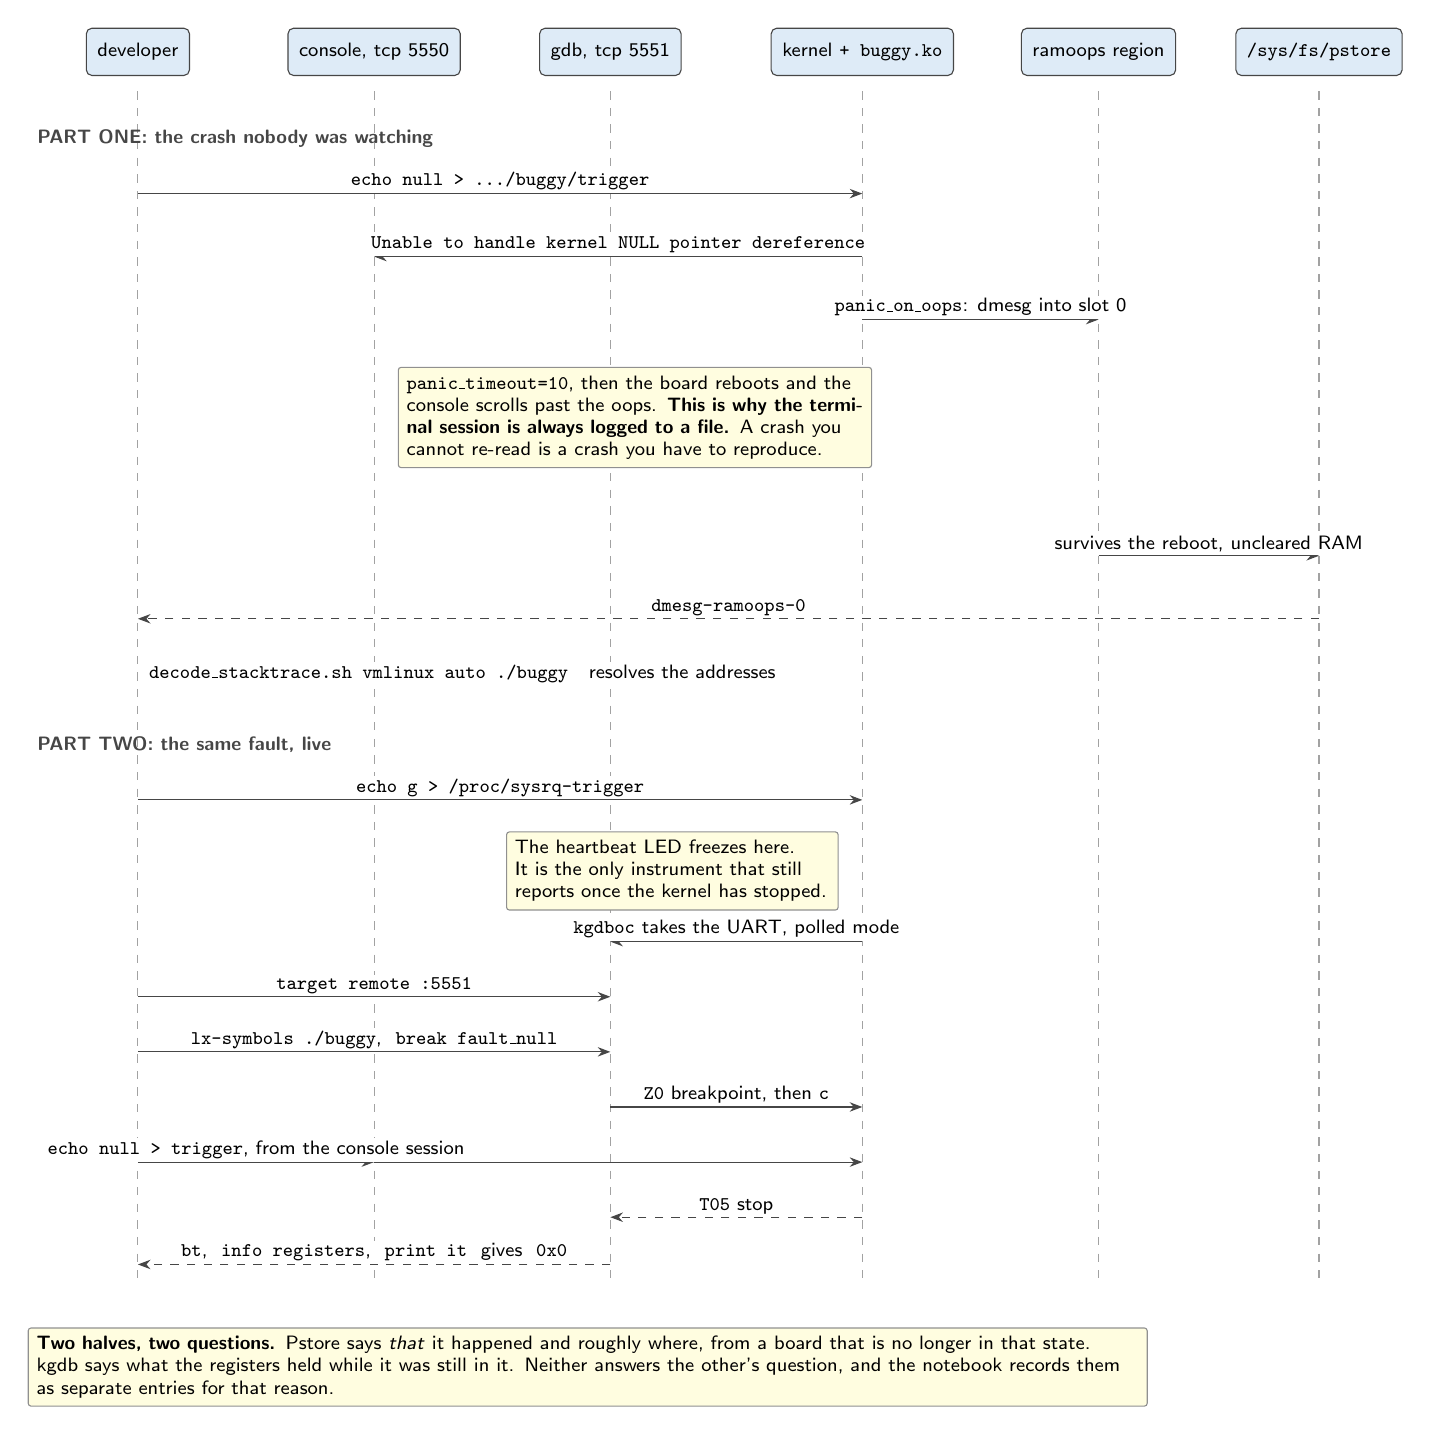
\begin{tikzpicture}[font=\sffamily\scriptsize]

  \def\ytop{0}
  \def\ybot{-15.6}

  %% ---------------- participants ----------------
  \foreach \x/\txt in {
      0/{developer},
      3.0/{console, tcp 5550},
      6.0/{gdb, tcp 5551},
      9.2/{kernel \texttt{+ buggy.ko}},
      12.2/{ramoops region},
      15.0/{\texttt{/sys/fs/pstore}}} {
    \node[actor] at (\x,\ytop) {\txt};
    \draw[lifeline] (\x,-0.5) -- (\x,\ybot);
  }

  %% ================ part one: nobody was watching ================
  \node[anchor=west, font=\sffamily\scriptsize\bfseries, text=linecol]
       at (-1.4,-1.1) {PART ONE: the crash nobody was watching};

  \draw[msg] (0,-1.8) -- node[lbl, above] {\texttt{echo null > .../buggy/trigger}} (9.2,-1.8);
  \draw[msg] (9.2,-2.6) -- node[lbl, above] {\texttt{Unable to handle kernel NULL pointer dereference}} (3.0,-2.6);
  \draw[msg] (9.2,-3.4) -- node[lbl, above] {\texttt{panic\_on\_oops}: dmesg into slot 0} (12.2,-3.4);

  \node[umlnote, anchor=north west, text width=58mm] at (3.3,-4.0)
       {\texttt{panic\_timeout=10}, then the board reboots and the console
        scrolls past the oops. \textbf{This is why the terminal session is
        always logged to a file.} A crash you cannot re-read is a crash you
        have to reproduce.};

  \draw[msg] (12.2,-6.4) -- node[lbl, above] {survives the reboot, uncleared RAM} (15.0,-6.4);
  \draw[reply] (15.0,-7.2) -- node[lbl, above] {\texttt{dmesg-ramoops-0}} (0,-7.2);
  \node[anchor=west, lbl] at (0.1,-7.9)
       {\texttt{decode\_stacktrace.sh vmlinux auto ./buggy} \ \ resolves the addresses};

  %% ================ part two: the same fault, live ================
  \node[anchor=west, font=\sffamily\scriptsize\bfseries, text=linecol]
       at (-1.4,-8.8) {PART TWO: the same fault, live};

  \draw[msg] (0,-9.5) -- node[lbl, above] {\texttt{echo g > /proc/sysrq-trigger}} (9.2,-9.5);
  \node[umlnote, anchor=north east, text width=40mm] at (8.9,-9.9)
       {The heartbeat LED freezes here. It is the only instrument that
        still reports once the kernel has stopped.};

  \draw[msg] (9.2,-11.3) -- node[lbl, above] {\texttt{kgdboc} takes the UART, polled mode} (6.0,-11.3);
  \draw[msg] (0,-12.0) -- node[lbl, above] {\texttt{target remote :5551}} (6.0,-12.0);
  \draw[msg] (0,-12.7) -- node[lbl, above] {\texttt{lx-symbols ./buggy}, \ \texttt{break fault\_null}} (6.0,-12.7);
  \draw[msg] (6.0,-13.4) -- node[lbl, above] {\texttt{Z0} breakpoint, then \texttt{c}} (9.2,-13.4);
  \draw[msg] (0,-14.1) -- node[lbl, above] {\texttt{echo null > trigger}, from the console session} (3.0,-14.1);
  \draw[msg] (3.0,-14.1) -- (9.2,-14.1);
  \draw[reply] (9.2,-14.8) -- node[lbl, above] {\texttt{T05} stop} (6.0,-14.8);
  \draw[reply] (6.0,-15.4) -- node[lbl, above] {\texttt{bt}, \ \texttt{info registers}, \ \texttt{print it} \ gives \ \texttt{0x0}} (0,-15.4);

  %% ---------------- the reading of it ----------------
  \node[umlnote, anchor=north west, text width=140mm] at (-1.4,-16.2)
       {\textbf{Two halves, two questions.} Pstore says \emph{that} it
        happened and roughly where, from a board that is no longer in that
        state. kgdb says what the registers held while it was still in it.
        Neither answers the other's question, and the notebook records them
        as separate entries for that reason.};

\end{tikzpicture}
\end{document}
